% !TEX root = BioInspired.tex

\chapter{Swarms - Text Chapter 5}

\section{ Problem 1 }
\textbf{Write a pseudocode for the simple ACO (S-ACO) algorithm considering pheromone evaportation, implement it computationally, and apply it to solve the TSP instance presented in Section 3.10.4. Discuss the results obtained.} \newline \\
\textbf{Remove the pheromone evaportation term (Equation ~\ref{eqn5.3}), apply the alogorithm to the same problem, and discuss the results obtained.}

\begin{equation} \label{eqn5.3}
\tau_{ij}(t) \leftarrow ( 1-\rho ) \tau_{ij}(t) + \Delta \tau
\end{equation}

% Problem 1 Discussion

\subsection{Summary}
The Traveling Salesman Problem is a popular problem in the field of computer science. The idea is there is a list of cities a salesman wants to visit, for the cheapest cost. In this problem, ant colony optomization is used to a find a low-cost solution.

\subsection{Implementation}
Code for this may be found in Listing~\ref{tsp_aco.cpp}.

The pseudocode for the simple ant colony optomization is presented in subsection ~\ref{acoPseudo}. This pseudocode has gone through a few revisions as code was written and moments of ``That's not going to work.'' occured. Currently, the code is written to read in cities locations from a file and create edges to form a complete graph with associated distances, pheromone, and visibilties. Next, a solution for each ant is built. A node is randomly selected for the starting point, a probability list (for moving to the next unvisited node) is constructed using Equation ~\ref{eqn5.5}, a random value is generated and checked against the probability list to see which node is next moved to. The selected node is then removed from the available nodes list, added to the visited list, and pheromone added to the edge. This repeats for each node until all nodes have been traversed.

\begin{equation} \label{eqn5.5}
p_{ij}^{k}(t) = 
	\begin{cases}
	\frac{ [\tau_{ij}(t)]^\alpha [\eta_{ij}]^\beta} {\Sigma_{l \in J_i^k}[\tau_{il}(t)]^\alpha[\eta_{il}]^\beta } & \text{if} j \in J_i^k \\
	0 	& \text{otherwise} \\
	\end{cases}
\end{equation}

Once the visited list for each ant has been built, the fitness of each path will be evaluated. To determine the fitness, it will simply be the total length of all edges. The most fit path will be the shortest path. Then, Equation ~\ref{eqn5.2} is applied to all edges to simulate the `evaporation' of pheromones. 

\begin{equation} \label{eqn5.2}
\tau_{ij}(t) \leftarrow \tau_i(t) + \Delta \tau
\end{equation}

\subsection{Analysis}
There's a bug in the bug code. A struct to contain edge information such as start node, end node, pheromone level, distance and visibilty was created. Then a 2D array of those structs was created to hold all possible edges. The 2D array is filled such that no edge is repeatedly stored, so half of the array is filled. Pheromone is intialized to one for all edges. 

During debugging of the move function, when accessing the pheromone information, occasionally the pheromone data would be 0 instead of 1. This could be an indexing issue, but on 3 hours of sleep, and checking the logic against several people, Stephanie can't figure out what's wrong. One would think that she would have learned from McGough's robotics class, his homeworks should really be started more than one week before it's due.

% S-ACO pseudocode
\subsection{ S-ACO Pseudocode } \label{acoPseudo}
\begin{lstlisting}
SACO( max_it, ants, edges )
{
	t = 0
	while ( t < max_it )
	{
		// for each ant
		// place ant on randomly selected node
		
		for( i = 0; ants; i++)
		{
			// calculate probability of moving to each untraveled node
			// use probabalistic move rule to determine next node
			// mark new node as traveled
			// add node to traveled path
		}
		
		// evaluate cost of each solution
		if ( solution < best )
			best = solution

		//update pheromone trails
		t++
	}
}
\end{lstlisting}


\section{ Problem 8 }
\textbf{Apply the PS algorithm described in Section 5.4.1 to the maximization problem of Example 3.3.3. Compare the relative performance of the PS algorithm with that obtained using a standard genetic algorithm.} \newline 

\subsection{Summary}
Expanding upon the evolutionary algorithms to solve the maximization problem of Example 3.3.3 in the book, a particle swarm approach is implemented and compared against the evoluationary algorithms.

\subsection{Implementation}
Random points along the x-axis between zero and one are initialized as the population. Each individual is then assigned a random initial velocity between zero and one. Next, each individual's fitness is then evaluated and the best fit individual is tracked. Then a loop is entered for a specified number of time steps. During each time step, each individual's velocity is slightly perturbed, the fitness re-evaluatated, and new best fit positions are tracked. The code can be found in Listing~\ref{pso.cpp}.

\subsection{Analysis}
The trials for this implementation were run with a population size of twenty and 500 time steps. With these conditions, the particle swarm successfully found the global max within a small tolerance each time it was run, see Figure ~\ref{psoRun} for some sample runs. Compared to the simple hill climbing algorithm, particle swarm will always find the global extrema, whereas the simple hill climber will not. So, particle swarm is better than the simple hill climber. The iterated and stochastic hill climbers consistently found the global extrema, so particle swarm is on par with them. The same can be said for the genetic algorithm.

Comments on run times can't be accurately made because python was used for some algorithms and c++ for the others. 

\begin{figure}[tbh]
\begin{center}
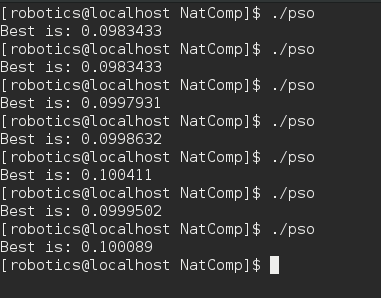
\includegraphics[width=0.5\textwidth]{psoRUN.png}
\end{center}
\caption{ Sample Particle Swarm Answers } \label{psoRun}
\end{figure}